\documentclass[titlepage]{article}
\usepackage[utf8]{inputenc}
\usepackage{graphicx}
\usepackage{hyperref}
\graphicspath{ {./images/} }

\title{\textbf{Battleship} \\ CS251 : Software Systems Lab}
\author{Rahul Bhardwaj, Anuj Diwan, Soumya Chatterjee \\ 170050012, 170070005, 170070010}
\date{November 2018}

\begin{document}

\maketitle

\tableofcontents

\break

\section{Introduction and Motivation}
\subsection{Introduction}
% About the project %
We have implemented an online version of the classic multiplayer game Battleship with a twist which can be played on a web browser. The game supports multiple simultaneous game sessions and has unconventional features like I, T and L shaped ships and timed attacks. Opponents are also provided with an interface through which they can chat while playing the game.

\subsection{Motivation}
Having worked with various different languages, frameworks and tools throughout our course `Software Systems Lab', we were eager to apply all that we had learnt to create something substantial and complete. The course project gave us the valuable opportunity to explore new frameworks while applying the knowledge and experience gained throughout the course.

Our main motivation behind taking up this project was to to get an experience of working on a Client Server architecture, WebSockets, learning database management, and webpage design. We also wanted to explore different communication protocols.

\section{Features}


\begin{enumerate}
  \item Signup and Login- We have added signup and login features with custom fields like biodata, birthdate, etc. to allow users to create accounts.
  \item Dynamic List of Players- A list of players who are ready to play can be seen by the users after logging in.
  \item User profile contains bio,location, total score, etc. and is viewable for each active player in the lobby.
  \item Players can send and receive play requests to and from any of the active players apart from himself/herself.
  \item The player to whom the request has been sent will get a pop-up asking him to accept/reject the request and upon acceptance both are redirected to another page where ships can be.
  \item I,L,T shaped ships are supported. The game checks that there are no overlapping and/or out-of-bounds ships.
  \item After correctly placing the ships, they are redirected to the play page.
  \item Players can chat on the game screen.
  \item The player whose turn it is can attack on the opponent's board. Timed attacks are used. States are updated on timeout and button. The game ends when all the ships of a player are destroyed.
  \item Since the game states are updated to and from the Django server, the game state is preserved on refresh, thus the full game loads on refresh.
  \item Scores of each player, and number of wins and games played is stored for each player. The leaderboard shows the players sorted by total points.
\end{enumerate}



% \section{Implementation Details}

\section{Software and Tools Used}
We used the Django development server for automatic handling of database operations and Redis server for using Django channels to establish persistent connections through websockets. SQlite was used for handling the database. Various Linux and Python packages were used as follows:
\begin{itemize}
    \item Linux
    \begin{itemize}
        \item Python Dev
        \item Redis
        \item Net Tools
    \end{itemize}
    \item Python
    \begin{itemize}
        \item Django == 2.1.3
        \item Django Crispy Forms == 1.7.2
        \item Channels == 2.1.5
        \item Django Picklefield == 1.1.0
        \item Channels-Redis == 2.3.1
    \end{itemize}
\end{itemize}

\begin{center}
\begin{figure}[h]
    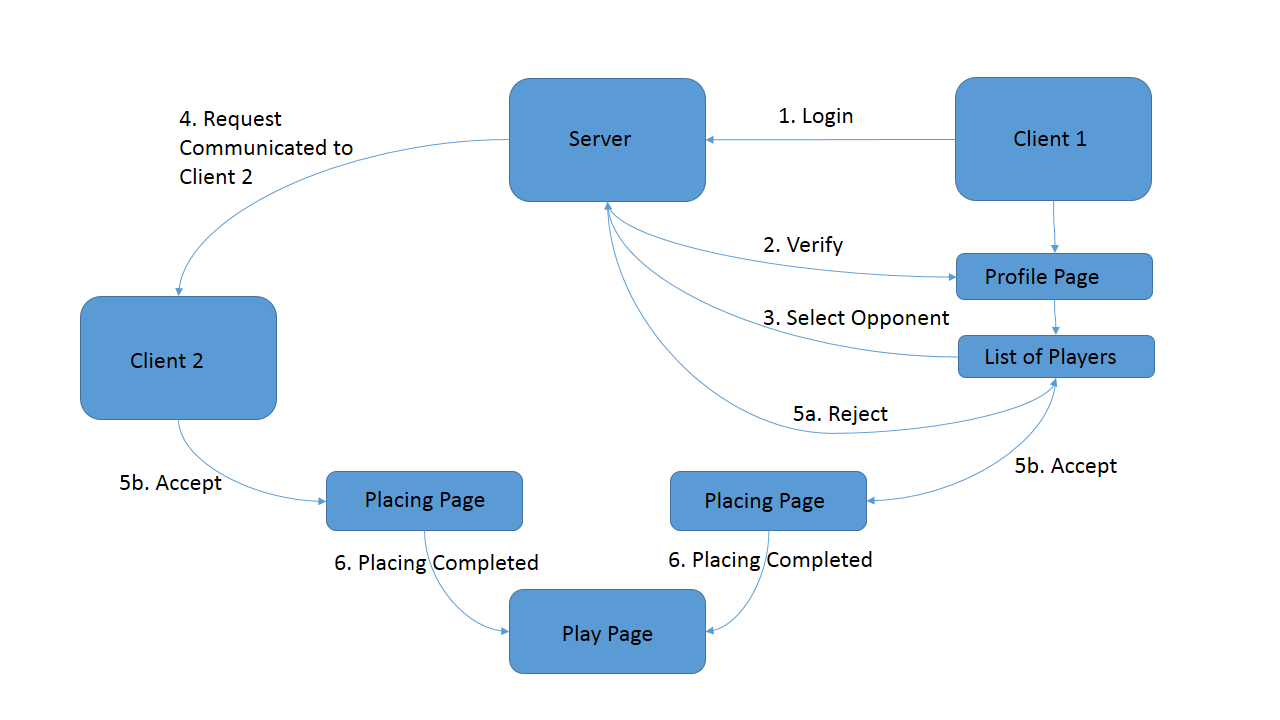
\includegraphics[scale=0.35]{Slide3.PNG}\\
    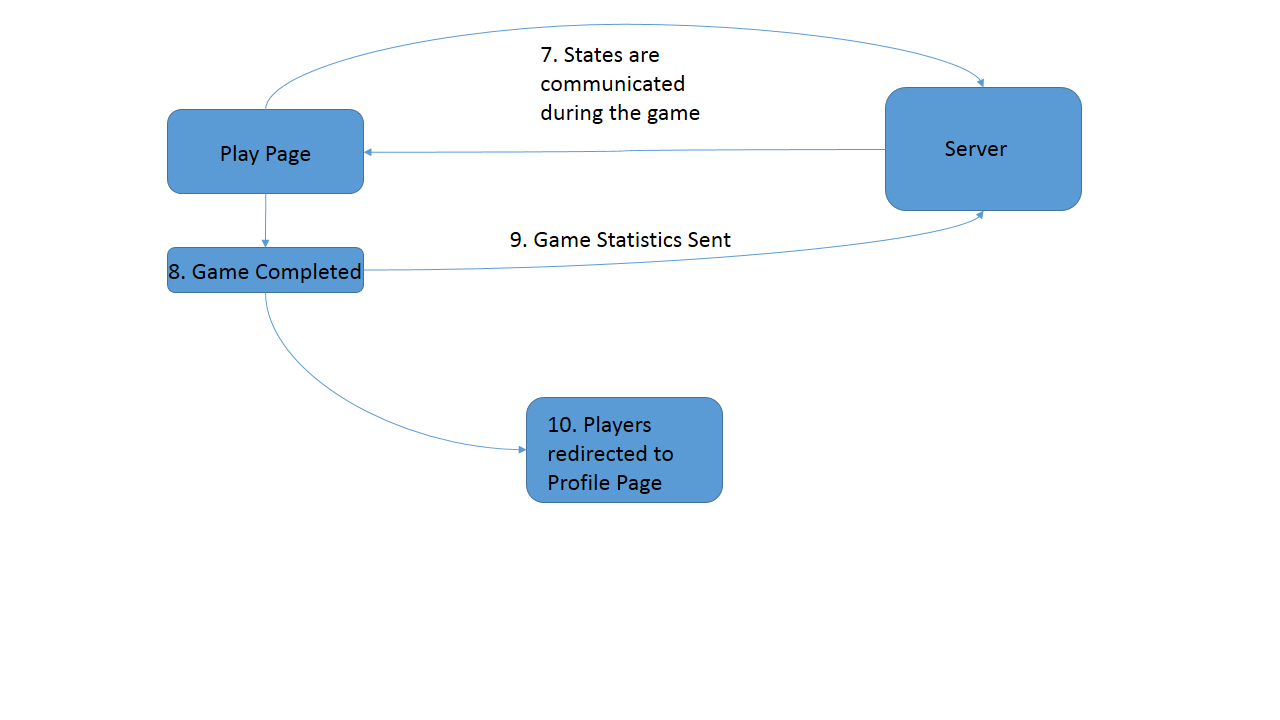
\includegraphics[scale=0.35]{Slide4.PNG}
\end{figure}
\end{center}


\section{Login and Logout Features}
The inbuilt django auth app was used to implement login, logout and and signup feature. The default form was used for login and logout and a custom form for signup. The custom signup form was built by extending the existing user creation form, with additional fields corresponding to those of the profile object. We used     django-crispy-forms to Bootstrap the forms.
\subsection{Signup}
The signup page was implemented by making a CustomSignupForm that extends the UserCreationForm. Additional fields for bio and location are created. The date-of-birth widget is implemented using a SelectDateWidget.
\section{Player List}
\subsection{Backend}
 The database handling was done using SQlite. We created a Profile class to store user objects which contains information like username, bio, location, date of birth and a boolean which store whether the player is currently available or not.

 We have defined 2 views in the pairing app - Profile view and the list view to see the list of players currently available. Upon logging in the user will be directed to the profile view, where he can click on 'Begin Game' which will take him to the listAvailable view. The list of players which are currently active will get updated automatically if a user logs out or begins playing(using websockets).

\subsection{Websocket Connection}
The list of players who are currently active (i.e. ready to play) needed to be updated automatically. To implement this, we established a web-socket connection by routing it to the Redis server and a persistent connection was formed along with associated consumer object. This was implemented using django channels. We wrote a consumer called ChatConsumer to handle the events of players sending, accepting and rejecting requests. When a user logins in, the information that the player now is available is sent to the entire group of channels and its isAvailable attribute is set to true. At the receiver's end the channel sends the message to the javascript handler. The same thing happens when a user logs out. For other types of messages(like Accept, Reject, Send, Cancel requests), the type of message that has been sent is stored in the purpose attribute of the message.

\subsubsection{Receiving and Handling Messages}
If the message contains the `loggedIn' attribute then it corresponds to a user logging in/out, the only action which will be performed is the list of users getting updated. If the message contains the logged\_in attribute with a True isLoggedIn attribute, we show that user also in the list, else we hide it.  On the other hand if the message does not contain the `loggedIn' attribute, then we check the purpose attribute of the message. If the purpose attribute is `Send Request', then we show the model displaying that a play request has been sent. If the purpose attribute is `Accept\_Request', then we display the message that his request was accepted by the other player and then direct them to the play pages. If the purpose attribute was "Reject\_Request", then we display a message saying that his request was rejected.  His decision will also be conveyed to the sender of the message. We handled all this using the javascript function \texttt{socket.onmessage} in \texttt{list.html}

\subsubsection{Sending Messages}
In the list.html we defined a function to handle the events of a user clicking on another user's profile and thereby sending a request. The message was again sent as a JSON containing `from', `to', `purpose' and `type' attributes. The javascript function sends this message over WebSocket to the ChatConsumer. The ChatConsumer upon receiving the message forwards it to the entire group of channels. This is done when a user sends or cancels a request. The ChatConsumers of the receiving channel then sends the message over websocket to javascript, which is then handled in the way described in the above paragraph.
\subsection{Leaderboard}
On the pairing page, a leaderboard of all users is displayed on the right. The leaderboard is sorted according to the total number of points each player has. In case two players have the same number of points, the number of games they have won are compared. This is implemented by first displaying all the users using the Django template language and storing the scores and the number of games won, and then sorting the list according to the given criterion.
\section{Placing Ships}
The front-end was implemented using the Javascript library React.
In the placing.html file we have created a class called board which will store the current state of the board and defined a function to handle the onclick event. It contains a variable to store which all squares on the board and another variable which stores the points which a particular ship covers. The render function is designed to display the board and give the user options to select ships and place them on the board. We have also created functions which handle events related to placing of ships. For all the ships, we have decided on keeping a point as pivot and then allowing rotations about that point. There are 4 possible orientations for every ship(though some of them may be same for a few pieces). Clicking on a ship selects it and clicking on it subsequent times, rotates it. The player can choose a ship, its orientation and the point where to keep its pivot, after which the function `handleClick' will be called. Based on the ship and its orientation we push all the points covered by that particular ship into an array and then check if any of them goes outside the board and if all the ships have been placed. If both these conditions are met, we send a message through the websocket to django in order to update the database. We also display the number of ships of each type which have been successfully placed.

\section{The Actual Game}
To enable communication between the players, we have again made use of websocket connections. As soon as the players get redirected to the play page, the socket connection gets established. Consumers.py contains a `SubmitConsumer' class, whose member functions handle various events related to the game. Upon page load a Websocket connection is established that receives the current state of the game from Django. This then renders the boards appropriately and also the scores. The colours and which player's turn it is are implemented using the render() functions of the Boards.

\subsection{Shooting}
The `game.html' file contains a Board class. It renders the board and also the number of ships which are left to be sunk by the current player. It has an HandleClick function, which when called updates all the info and sends a message to django in order to update the state. Django on receiving the message updates the corresponding game object and the sends the message to javascript and also back to the group, indicating that the data has been updated.
For handling the message at the receiver's end, we have \texttt{socket.onmessage} function, which gets called when a message is received. It then internally calls updateState, which updates information like the state of the board and the current player after checking whether the player receiving the message is player 1 or player 2.

\subsection{Chat Interface between players}
The idea is again almost the same. `Consumers.py' contains a class named `GameChatConsumer' to handle chat messages.Connect and disconnect functions handle joining and leaving of players from the chat room. The reciev function on recieving from the websocket echoes the message to the entire group. The chat message function on recieving a message check if the purpose attribute is `Game\_Chat' and if the game\_is equal to self.game\_id, in which case, it sends the message to the javascript. To handle the javascript part we have defined a class called GameChat. The class contains 2 string array's in it state. One of them store the messages and the other stores the sender. It componentDidMount functions handles the receiving of messages. When a message is recieved through the websocket, it pushes the message and sender into the respective arrays. The render function of the class displays the message the along with the senders.
\section{Contributions}
\subsection{Anuj}
    \begin{itemize}
        \item Making all the models for the backend database(profile model, game model) and the logic for handling login and logout. Making the custom signup form and implementing the widget for the birthdate.
        \item Implemented the persistent connection logic in Django using django-channels and the Websocket and Javascript logic for displaying active players in the list and sending and accepting requests.
        \item Implemented the logic for removing players when they are in the process of connecting(modals are on screen) and readding them when the modals disappear.
        \item The code for showing the leaderboard of all the users.
        \item Designing and implementing the collision, out-of-bounds, and placing logic for placing the ships. Also the sending of state to Django on submit. Wrote the consumer classes for handling placing requests and game requests.
        \item Implemented the game state update and sending(storing board squares, sunk ships, etc.) to Django using Javascript.
        This required a complex checking of the board state and appropriate update under various circumstances.
        \item Wrote the logic for recording the number of sunk ships and displaying it on the page.
        \item Enabled persistent game state by storing the state in Django itself. Used CSS and HTML for the in-nav-bar score and designed the page layout on the game page, including the two boards and the colour changes of the two boards.
        \item Made the countdown timer for timed attacks and handled it appropriately. Also made the scoring logic work.
        \item Made the code work for multiple matches. Designed the final page(game over page).
        \item Wrote the \LaTeX \ report.
    \end{itemize}

\subsection{Soumya}
    \begin{itemize}
        \item Implemented the persistent connections of the player listing page using Websockets in Django using django-channels and wrote the consumer classes required to handle the messages from the sockets
        \item The Javascript logic for displaying active players in the list and sending and accepting requests. Wrote the Javascript functions to handle game pairing requests from a user and forward it to the desired user
        \item Worked on the Profile model for storing the user attributes in Django
        \item Displaying the attributes of users on the profile page and in the lobby.
        \item Implemented the in-game chat interface and created the required Websockets and Consumer classes for handling the same
        \item Designing and implementing the layout of all the pages using Bootstrap and CSS.
        \item Designing the grid, buttons of the grid and the buttons used to choose which ship to place, including the rotation animation and the colours etc. Used React for the dynamic rendering of the grid and related components
        \item Worked on some parts of the game state handling in Javascript and also on the timed moves
        \item Wrote various JQuery scripts for handling diverse operation like selecting DOM elements for changing their states
        \item Wrote the shell scripts for installing all the required dependencies and setting up the game server to allow multiple users on the same network to play the game
        \item Wrote the README.md file(the user manual) and the \LaTeX\space Report.
    \end{itemize}
\subsection{Rahul}
    \begin{itemize}
        \item Implementing sending of state of placed ships to Django when the user clicks on the submit button on the placing pages in order to update information about the game object.
        \item Designed and implemented the chat application on the game page which required sending the messages to django thorugh a websocket.
        \item Wrote the React code for rendering all the messages of both the users and dynamically maintaining all the messages and their senders as part of the Chat Consumer class.
        \item Wrote the Graphical User Interface part of displaying the count of the ships on the placing page and the game page.
        \item Wrote the React code for displaying the buttons for this ships on the placing page.
        \item Wrote the React code for rendering the board of both the players on the game page and displaying the relevant information.
        \item Ran the shell script on a VM to make sure it works.
        \item Wrote the \LaTeX\space documentation covering all the technical details of the project and depicting how each part of the project was implemented.
        \item Made the presentation covering all the features of the game implemented along with directions on how to use it.
    \end{itemize}

\section{References}
\begin{enumerate}
    \item \href{https://stackoverflow.com/}{https://stackoverflow.com/}
    \item \href{https://docs.djangoproject.com/en/2.1/}{https://docs.djangoproject.com/en/2.1/}
    \item \href{https://channels.readthedocs.io/en/latest/}{https://channels.readthedocs.io/en/latest/}
    \item \href{https://hackernoon.com/reconciling-djangos-mvc-templates-with-react-components-3aa986cf510a}{https://hackernoon.com/reconciling-djangos-mvc-templates-with-react-components-3aa986cf510a}
    \item \href{https://realpython.com/getting-started-with-django-channels/}{https://realpython.com/getting-started-with-django-channels/}
    \item \href{https://blog.heroku.com/in_deep_with_django_channels_the_future_of_real_time_apps_in_django}{https://blog.heroku.com/in\_deep\_with\_django\_channels\_the\_future\_of\_real\_time\_apps\_in\_django}
    \item \href{https://medium.com/practo-engineering/websockets-in-react-the-component-way-368730334eef}{https://medium.com/practo-engineering/websockets-in-react-the-component-way-368730334eef}
    \item \href{https://reactjs.org/tutorial/tutorial.html}{https://reactjs.org/tutorial/tutorial.html}
    \item \href{https://codeburst.io/lets-build-a-countdown-timer-with-react-part-1-2e7d5692d914}{https://codeburst.io/lets-build-a-countdown-timer-with-react-part-1-2e7d5692d914}
\end{enumerate}
\end{document}
